\usepackage{graphicx}
\usepackage{amssymb}
\usepackage{xparse}

\input{macros/sets}
\input{macros/category}
\input{macros/circuits}
\input{macros/streams}

\graphicspath{{./imgs/}}

\usetheme[
  background=light,
  numbering=counter,
  block=fill,
  %sectionpage=simple
]{metropolis}

% FiraFonts
\usepackage[sfdefault]{FiraSans}
\usepackage{FiraMono}
% Use thinner fonts
\makeatletter
\def\bfseries@sf{medium}
\def\mdseries@sf{l}
\makeatother

\definecolor{backg}{RGB}{9,72,61}
\definecolor{accent}{RGB}{0,150,136}

\definecolor{dracback}{RGB}{40, 42, 54}
\definecolor{dracfore}{RGB}{248, 248, 242}
\definecolor{dractitle}{RGB}{56, 58, 89}
\definecolor{dracblock}{RGB}{98, 114, 164}
\definecolor{draccent}{RGB}{255, 121, 198}

\setbeamercolor{normal text}{bg=dracfore}
\setbeamercolor{frametitle}{bg=dractitle, fg=dracfore}
\setbeamercolor{title separator}{fg=draccent}
\setbeamercolor{progress bar}{fg=draccent, bg=draccent}
\setbeamercolor{block title}{fg=dracfore, bg=dracblock}
\setbeamercolor{alerted text}{fg=draccent}

\newtheorem{axiom}{Axiom(s)}

\title{A compositional theory of digital circuits}
\author{
    \texorpdfstring{
        \large\textbf{George Kaye} \\[0.25em]
        \footnotesize University of Birmingham
    }{
        George Kaye
    }
}
\date{
    05 April 2023
}

\begin{document}
    \maketitle
    \begin{frame}
    \frametitle{What are we going to be talking about?}
    \pause
    \centering
    \LARGE
    Digital circuits!

    
\includegraphics[width=0.6\textwidth]{imgs/circuit}
\end{frame}
\begin{frame}
    \frametitle{What are we going to be talking about?}
    \centering
    \LARGE
    Digital circuits!

    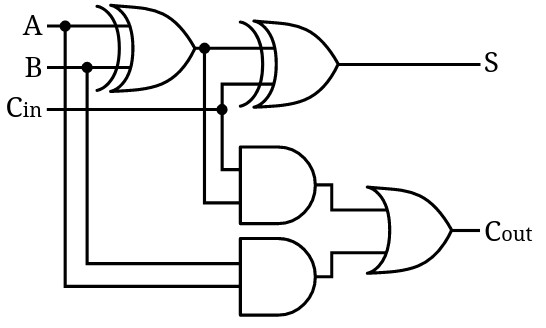
\includegraphics[width=0.6\textwidth]{imgs/adder}
\end{frame}
\begin{frame}
    \frametitle{What are we going to be talking about?}

    \pause

    \centering
    \LARGE
    We want a \alert{compositional} theory of digital circuits.

    \vspace{0.5em}

    \normalsize

    \pause
    F g

    \vspace{0.5em}
    Composites

    \pause
    \vspace{0.5em}

\end{frame}
\begin{frame}
    \frametitle{But why do we want that?}
    \centering
    \LARGE
    We want to reason \alert{equationally} about circuits.

    \normalsize
    Example rewrite of circuits (definition of rewrite will do)

\end{frame}
\begin{frame}
    \frametitle{Why all the pictures?}
    \centering
    \LARGE
    String diagrams are \alert{good}.

    \normalsize
    (but these are a little different to the ones Dan and Jamie are using)

    put some pictures on this slide too

\end{frame}
    \begin{frame}
    \frametitle{I thought this was about circuits}

    \centering

    \pause
    \svg{0}{1}{and}
    \pause\quad
    \svg{0}{1}{or}
    \pause\quad
    \svg{0}{1}{not}

    \vspace{1em}

    \pause
    \svg{0}{1}{fork}
    \pause\quad
    \svg{0}{1}{join}
    \pause\quad
    \svg{0.5}{1}{stub}
    \pause\quad
    \svg{0.5}{1}{init}

\end{frame}
\begin{frame}
    \frametitle{Putting the pieces together}

    \centering
    \LARGE
    This lets us build \alert{combinational} circuits.

    \vspace{1em}
    \normalsize
    \svg{-1}{0.75}{xor}
    \quad\(:=\)\quad
    \svg{-3}{0.75}{xor-def}

\end{frame}
\begin{frame}
    \frametitle{Putting the pieces together}

    \centering
    \LARGE
    These circuits are \alert{boring}!
    \pause
    Circuits need \alert{state}...

    \normalsize
    \vspace{1em}

    \pause
    \svg{0}{1}{true}
    \pause\quad
    \svg{0}{1}{false}
    \pause\quad
    \svg{0}{1}{both}
    \pause\quad
    \svg{0}{1}{delay}

    \pause
    \vspace{1em}

    \LARGE
    ...and \alert{feedback}!
    \normalsize

    \vspace{1em}
    \pause

    \svg{-1.5}{1}{h}
    \pause
    \quad\(\rightarrow\)\quad
    \svg{-1.5}{1}{trace}
\end{frame}
    \begin{frame}
    \frametitle{This is all very pretty but...}

    \centering

    \LARGE
    Now what?

    \pause

    None of this means anything!

\end{frame}
\begin{frame}
    \frametitle{Open the gates}

    \centering
    \svg{0}{1}{gate-eqs}

\end{frame}
\begin{frame}
    \frametitle{Fork in the road}

    \centering
    \svg{0}{1.25}{fork-eqs}

\end{frame}
\begin{frame}
    \frametitle{Time to join up}

    \centering
    \svg{0}{0.75}{join-eqs}

\end{frame}
\begin{frame}
    \frametitle{This article is a stub}

    \centering
    \svg{0}{1.25}{stub-eqs}

\end{frame}
\begin{frame}
    \frametitle{Did we get it right?}

    \centering
    \LARGE
    true \alert{XOR} false

    \normalsize

    \visible<2>{\only<1-2>{\svg{0}{1}{xor-test-1}}}%
    \only<3>{\svg{0}{1}{xor-test-2}}%
    \only<4>{\svg{0}{1}{xor-test-3}}%
    \only<5>{\svg{0}{1}{xor-test-4}}%
    \only<6>{\svg{0}{1}{xor-test-5}}%

\end{frame}
\begin{frame}
    \frametitle{We must not delay}

    \centering
    \svg{0}{1.25}{delay-eqs}

\end{frame}
\begin{frame}
    \frametitle{This gives us some nice structure}

    \centering
    \LARGE

    \pause

    From \alert{axioms} we derive \alert{theorems}

    \pause
    \vspace{1em}

    \svg{0}{0.75}{copy}

    \pause

    \vspace{1em}

    \svg{0}{0.75}{discard}

\end{frame}
\begin{frame}
    \frametitle{Trust the process}

    \pause
    \LARGE
    \centering
    We want to \alert{process} inputs to obtain \alert{outputs}
    \normalsize

    \pause
    \vspace{1em}

    \svg{0}{1}{productivity}

\end{frame}
\begin{frame}
    \frametitle{This axiom is the last one}

    \pause
    \centering
    \svg{0}{0.8}{streaming}

    \vspace{1em}
    \pause

    \svg{0}{0.8}{gen-streaming}

\end{frame}
\begin{frame}
    \frametitle{A big(ish) example}

    \centering
    \only<1>{\svg{0}{0.75}{acc}}%
    \only<2>{\svg{0}{0.75}{acc-1}}%
    \only<3>{\svg{0}{0.75}{acc-2}}%
    \only<4>{\svg{0}{0.75}{acc-3}}%
    \only<5>{\svg{0}{0.75}{acc-4}}%
    \only<6>{\svg{0}{0.75}{acc-5}}%
    \only<7>{\svg{0}{0.75}{acc-6}}%

\end{frame}
\begin{frame}
    \frametitle{We made it!}

    \centering

    \LARGE
    We're only scratching the surface!

    \vspace{1em}

    \large
    \pause

    \alert{Arbitrary} gate and value sets...

    \pause

    Handling \alert{non-delay-guarded feedback}...

    \pause

    Defining the \alert{denotational semantics} of circuits as stream functions...

    \pause
    Interpreting circuits as \alert{hypergraphs} for reasoning computationally...

    \pause
    \vspace{1em}

    \scriptsize
    (someone could write this up as a PhD thesis)

\end{frame}
\end{document}